\chapter{Leçon 30: Virstellungen an e Bild beschreiwen}

Dës Lektioun beschäftegt sech mat de perséinleche Virstellungen vun eise Studenten an der Beschreiwung vun engem Bild op der Tafel. Mir studéieren d'lokal Prepositiounen mat dem Dativ (\textbf{lénks/riets vum}, \textbf{an der Mëtt}, \textbf{virun}, \textbf{hannert}, \textbf{niewent}, \textbf{ënner/ënnert}, \textbf{iwwer/iwwert}, \textbf{tëschent}) an d'Konstruktioun vun der Beschreiwung am Lëtzebuergeschen. Mir kucken och d'Spillereien vun der Aussprooch mat dem Witz vum \textbf{schéinen Dag} géint de \textbf{schéinen Daach}. \textit{Cette leçon porte sur les présentations personnelles de nos étudiants et sur la description d'une image au tableau. Nous étudions les prépositions de lieu suivies du datif (\textbf{lénks/riets vum} - à gauche/droite de, \textbf{an der Mëtt} - au milieu, \textbf{virun} - devant, \textbf{hannert} - derrière, \textbf{niewent} - à côté de, \textbf{ënner/ënnert} - sous, \textbf{iwwer/iwwert} - sur/au-dessus de, \textbf{tëschent} - entre) et la construction de la description en luxembourgeois. Nous abordons également les particularités de prononciation avec la plaisanterie entre \textbf{schéinen Dag} (bonne journée) et \textbf{schéinen Daach} (beau toit). / This lesson covers personal introductions of our students and describing a picture on the whiteboard. We study prepositions of place governing the dative case (\textbf{lénks/riets vum} - to the left/right of, \textbf{an der Mëtt} - in the middle, \textbf{virun} - in front of, \textbf{hannert} - behind, \textbf{niewent} - next to, \textbf{ënner/ënnert} - under, \textbf{iwwer/iwwert} - above, \textbf{tëschent} - between) and the structure of descriptions in Luxembourgish. We also look at wordplay with the joke about \textbf{schéinen Dag} (nice day) vs \textbf{schéinen Daach} (beautiful roof).}

\vspace{1em}

\section[Dialog: Virstellungen an d'Bild op der Tafel / Dialogue / Dialogue]{Dialog: Virstellungen an d'Bild op der Tafel \\/ Dialogue : Présentations et description d'image \\/ Dialogue: Introductions and Picture Description}

Biergerlech Informatiounen iwwer d'Studenten an dësem Dialog sinn fiktiv. \\
\textit{Note : Les informations personnelles sur les étudiants dans ce dialogue sont fictives. / Note: The personal information about the students in this dialogue is fictional.}

\vspace{1.5em}

\noindent\textbf{1. Odile: Moien alleguer! Haut wëlle mir eis kuerz virstellen, well mir nei Leit an eisem Cours hunn. Wien fänkt un?}\\
\textit{Moien alleguer} (Bonjour tout le monde / Hello everyone)! \textit{Haut wëlle mir eis} (aujourd'hui nous voulons nous / today we want to) \textit{kuerz virstellen} (présenter brièvement / introduce briefly), \textit{well mir} (parce que nous / because we) \textit{nei Leit} (de nouvelles personnes / new people) \textit{an eisem Cours hunn} (avons dans notre cours / have in our class). \textit{Wien fänkt un} (Qui commence / Who starts)?\\
$\rightarrow$ Français : \textit{Bonjour tout le monde ! Aujourd'hui nous voulons nous présenter brièvement, car nous avons de nouvelles personnes dans notre cours. Qui commence ?}\\
$\rightarrow$ English : \textit{Hello everyone! Today we want to introduce ourselves briefly, because we have new people in our class. Who starts?}\\[0.5em]

\noindent\textbf{2. Josiane: Ech fänken un. Moien alleguer, ech heesche Josiane. Ech si pensionéiert. Fréier war ech Buschauffer an hunn an der Economie an am Sozialberäich geschafft. Ech sinn net bestuet an hu keng Kanner. Meng Mammesprooch ass Lëtzebuergesch. Ech wunnen a si gebuer zu Beetref. Ech hu stänneg eng Kaz doheem, de Simba.}\\
\textit{Ech fänken un} (Je commence / I start). \textit{Moien alleguer} (Bonjour à tous / Hello everyone), \textit{ech heesche Josiane} (je m'appelle Josiane / my name is Josiane). \textit{Ech si pensionéiert} (Je suis retraitée / I am retired). \textit{Fréier war ech} (Autrefois j'étais / In the past I was) \textit{Buschauffer} (chauffeur de bus / bus driver) \textit{an hunn an der Economie} (et ai travaillé dans l'économie / and worked in economics) \textit{an am Sozialberäich geschafft} (et dans le domaine social / and in the social sector). \textit{Ech sinn net bestuet} (Je ne suis pas mariée / I am not married) \textit{an hu keng Kanner} (et n'ai pas d'enfants / and have no children). \textit{Meng Mammesprooch} (Ma langue maternelle / My mother tongue) \textit{ass Lëtzebuergesch} (est le luxembourgeois / is Luxembourgish). \textit{Ech wunnen} (J'habite / I live) \textit{a si gebuer} (et suis née / and was born) \textit{zu Beetref} (à Bettendorf / in Bettendorf). \textit{Ech hu stänneg} (J'ai constamment / I constantly have) \textit{eng Kaz doheem} (un chat à la maison / a cat at home), \textit{de Simba} (Simba).\\
$\rightarrow$ Français : \textit{Je commence. Bonjour à tous, je m'appelle Josiane. Je suis retraitée. Autrefois, j'étais chauffeur de bus et j'ai travaillé dans l'économie et dans le domaine social. Je ne suis pas mariée et je n'ai pas d'enfants. Ma langue maternelle est le luxembourgeois. J'habite et je suis née à Bettendorf. J'ai toujours un chat à la maison, Simba.}\\
$\rightarrow$ English : \textit{I will start. Hello everyone, my name is Josiane. I am retired. In the past, I was a bus driver and I worked in economics and in the social sector. I am not married and have no children. My mother tongue is Luxembourgish. I live and was born in Bettendorf. I constantly have a cat at home, Simba.}\\[0.5em]

\noindent\textbf{3. Senada: Moien, ech heesche Senada. Ech kommen aus Jugoslawien, aus Serbien. Ech wunnen zanter dräizéng Joer zu Jonglënster. Ech schaffen als Botzfra an enger Schoul an der Hëllef. Ech hu dräi Kanner: zwee Meedercher an ee Jong, déi scho bestuet sinn. Meng Mammesprooch ass Serbesch, mee ech schwätzen och Däitsch, Franséisch, Albanesch, Russesch, Kroatesch, Bosnesch a bëssen Englesch.}\\
\textit{Moien} (Bonjour / Hello), \textit{ech heesche Senada} (je m'appelle Senada / my name is Senada). \textit{Ech kommen aus Jugoslawien} (Je viens de Yougoslavie / I come from Yugoslavia), \textit{aus Serbien} (de Serbie / from Serbia). \textit{Ech wunnen zanter dräizéng Joer} (J'habite depuis treize ans / I have lived for thirteen years) \textit{zu Jonglënster} (à Junglinster / in Junglinster). \textit{Ech schaffen als Botzfra} (Je travaille comme femme de ménage / I work as a cleaning lady) \textit{an enger Schoul} (dans une école / in a school) \textit{an der Hëllef} (dans l'assistance / in helper staff). \textit{Ech hunn dräi Kanner} (J'ai trois enfants / I have three children): \textit{zwee Meedercher} (deux filles / two daughters) \textit{an ee Jong} (et un garçon / and one son), \textit{déi scho bestuet sinn} (qui sont déjà mariés / who are already married). \textit{Meng Mammesprooch} (Ma langue maternelle / My mother tongue) \textit{ass Serbesch} (est le serbe / is Serbian), \textit{mee ech schwätzen och} (mais je parle aussi / but I also speak) \textit{Däitsch, Franséisch, Albanesch, Russesch, Kroatesch, Bosnesch a bëssen Englesch} (l'allemand, le français, l'albanais, le russe, le croate, le bosnien et un peu d'anglais).\\
$\rightarrow$ Français : \textit{Bonjour, je m'appelle Senada. Je viens de Yougoslavie, de Serbie. J'habite depuis treize ans à Junglinster. Je travaille comme femme de ménage auxiliaire dans une école. J'ai trois enfants : deux filles et un garçon, qui sont déjà mariés. Ma langue maternelle est le serbe, mais je parle aussi allemand, français, albanais, russe, croate, bosnien et un peu anglais.}\\
$\rightarrow$ English : \textit{Hello, my name is Senada. I come from Yugoslavia, from Serbia. I have lived in Junglinster for thirteen years. I work as an assistant cleaning lady in a school. I have three children: two daughters and one son, who are already married. My mother tongue is Serbian, but I also speak German, French, Albanian, Russian, Croatian, Bosnian, and a little English.}\\[0.5em]

\noindent\textbf{4. Beatriz: Moien, ech heesche Beatriz. Ech kommen aus Mexiko. Ech wunnen zanter néng Joer hei zu Lëtzebuerg. Ech schaffen als Sekretärin. Meng Mammesprooch ass Spuenesch, mee ech schwätzen och Däitsch, Englesch a fir de Moment léieren ech Lëtzebuergesch.}\\
\textit{Moien} (Bonjour / Hello), \textit{ech heesche Beatriz} (je m'appelle Beatriz / my name is Beatriz). \textit{Ech kommen aus Mexiko} (Je viens du Mexique / I come from Mexico). \textit{Ech wunnen zanter néng Joer} (J'habite depuis neuf ans / I have lived for nine years) \textit{hei zu Lëtzebuerg} (ici au Luxembourg / here in Luxembourg). \textit{Ech schaffen als Sekretärin} (Je travaille comme secrétaire / I work as a secretary). \textit{Meng Mammesprooch} (Ma langue maternelle / My mother tongue) \textit{ass Spuenesch} (est l'espagnol / is Spanish), \textit{mee ech schwätzen och} (mais je parle aussi / but I also speak) \textit{Däitsch, Englesch} (l'allemand, l'anglais / German, English) \textit{a fir de Moment} (et pour le moment / and at the moment) \textit{léieren ech Lëtzebuergesch} (j'apprends le luxembourgeois / I am learning Luxembourgish).\\
$\rightarrow$ Français : \textit{Bonjour, je m'appelle Beatriz. Je viens du Mexique. J'habite ici au Luxembourg depuis neuf ans. Je travaille comme secrétaire. Ma langue maternelle est l'espagnol, mais je parle aussi allemand, anglais et pour le moment j'apprends le luxembourgeois.}\\
$\rightarrow$ English : \textit{Hello, my name is Beatriz. I come from Mexico. I have lived here in Luxembourg for nine years. I work as a secretary. My mother tongue is Spanish, but I also speak German, English, and at the moment I am learning Luxembourgish.}\\[0.5em]

\noindent\textbf{5. Carlos: Moien, ech heesche Carlos. Ech kommen aus Venezuela a wunnen hei zanter fast drësseg Joer. Ech schaffen och an der Schoul zu Jonglënster. Ech hu dräi Kanner: zwee Meedercher an ee Jong. Ech schwätzen Spuenesch, Franséisch, Hebräesch a Lëtzebuergesch.}\\
\textit{Moien} (Bonjour / Hello), \textit{ech heesche Carlos} (je m'appelle Carlos / my name is Carlos). \textit{Ech kommen aus Venezuela} (Je viens du Venezuela / I come from Venezuela) \textit{a wunnen hei} (et j'habite ici / and I live here) \textit{zanter fast drësseg Joer} (depuis presque trente ans / for almost thirty years). \textit{Ech schaffen och} (Je travaille aussi / I also work) \textit{an der Schoul zu Jonglënster} (à l'école de Junglinster / at the school in Junglinster). \textit{Ech hunn dräi Kanner} (J'ai trois enfants / I have three children): \textit{zwee Meedercher an ee Jong} (deux filles et un garçon / two daughters and one son). \textit{Ech schwätzen} (Je parle / I speak) \textit{Spuenesch, Franséisch, Hebräesch a Lëtzebuergesch} (l'espagnol, le français, l'hébreu et le luxembourgeois).\\
$\rightarrow$ Français : \textit{Bonjour, je m'appelle Carlos. Je viens du Venezuela et j'habite ici depuis presque trente ans. Je travaille aussi à l'école de Junglinster. J'ai trois enfants : deux filles et un garçon. Je parle espagnol, français, hébreu et luxembourgeois.}\\
$\rightarrow$ English : \textit{Hello, my name is Carlos. I come from Venezuela and I have lived here for almost thirty years. I also work at the school in Junglinster. I have three children: two daughters and one son. I speak Spanish, French, Hebrew, and Luxembourgish.}\\[0.5em]

\noindent\textbf{6. Antoine: Moien, ech heeschen Antoine. Ech si fënnefanzwanzeg Joer al a kommen aus Frankräich. Ech schaffen als Educateur an der Maison Relais zu Jonglënster. Ech schwätze Franséisch an Englesch an ech léieren elo Lëtzebuergesch.}\\
\textit{Moien} (Bonjour / Hello), \textit{ech heeschen Antoine} (je m'appelle Antoine / my name is Antoine). \textit{Ech si fënnefanzwanzeg Joer al} (J'ai 25 ans / I am 25 years old) \textit{a kommen aus Frankräich} (et je viens de France / and come from France). \textit{Ech schaffen als Educateur} (Je travaille comme éducateur / I work as an educator) \textit{an der Maison Relais zu Jonglënster} (à la Maison Relais de Junglinster / at the Maison Relais in Junglinster). \textit{Ech schwätze Franséisch an Englesch} (Je parle français et anglais / I speak French and English) \textit{an ech léieren elo Lëtzebuergesch} (et j'apprends maintenant le luxembourgeois / and I am learning Luxembourgish now).\\
$\rightarrow$ Français : \textit{Bonjour, je m'appelle Antoine. J'ai vingt-cinq ans et je viens de France. Je travaille comme éducateur à la Maison Relais de Junglinster. Je parle français et anglais, et maintenant j'apprends le luxembourgeois.}\\
$\rightarrow$ English : \textit{Hello, my name is Antoine. I am twenty-five years old and I come from France. I work as an educator at the Maison Relais in Junglinster. I speak French and English, and now I am learning Luxembourgish.}\\[0.5em]

\noindent\textbf{7. Andriy: Moien, ech heeschen Andriy. Ech si véierandrësseg Joer al. Ech kommen aus der Ukrain. Ech schaffen als IT-Spezialist. Meng Mammesprooch ass Russesch. Ech hunn zwee Muppen doheem: de Kano an d'Kira.}\\
\textit{Moien} (Bonjour / Hello), \textit{ech heeschen Andriy} (je m'appelle Andriy / my name is Andriy). \textit{Ech si véierandrësseg Joer al} (J'ai 34 ans / I am 34 years old). \textit{Ech kommen aus der Ukrain} (Je viens d'Ukraine / I come from Ukraine). \textit{Ech schaffen als IT-Spezialist} (Je travaille comme spécialiste informatique / I work as an IT specialist). \textit{Meng Mammesprooch} (Ma langue maternelle / My mother tongue) \textit{ass Russesch} (est le russe / is Russian). \textit{Ech hunn zwee Muppen} (J'ai deux chiens / I have two dogs) \textit{doheem} (à la maison / at home): \textit{de Kano an d'Kira} (Kano et Kira / Kano and Kira).\\
$\rightarrow$ Français : \textit{Bonjour, je m'appelle Andriy. J'ai trente-quatre ans. Je viens d'Ukraine. Je travaille comme spécialiste en informatique. Ma langue maternelle est le russe. J'ai deux chiens à la maison : Kano et Kira.}\\
$\rightarrow$ English : \textit{Hello, my name is Andriy. I am thirty-four years old. I come from Ukraine. I work as an IT specialist. My mother tongue is Russian. I have two dogs at home: Kano and Kira.}\\[0.5em]

\noindent\textbf{8. Odile: Wëllkomm alleguer! Dat ass e ganz interkulturelle Grupp. Odile ass mäin Numm, ech sinn och pensionéiert an ech leeden dëse Cours. Elo, kuckt wgl. op d'Tafel. Do ass e Bild. Wat gesi mir do? Beatriz, wat gesäit een do op der Tafel?}\\
\textit{Wëllkomm alleguer} (Bienvenue à tous / Welcome everyone)! \textit{Dat ass} (C'est / That is) \textit{e ganz interkulturelle Grupp} (un groupe très interculturel / a very intercultural group). \textit{Odile ass mäin Numm} (Odile est mon nom / Odile is my name), \textit{ech sinn och pensionéiert} (je suis aussi retraitée / I am also retired) \textit{an ech leeden dëse Cours} (et je dirige ce cours / and I lead this class). \textit{Elo, kuckt wgl.} (Maintenant, regardez s'il vous plaît / Now, please look) \textit{op d'Tafel} (au tableau / at the board). \textit{Do ass e Bild} (Là est une image / There is a picture). \textit{Wat gesi mir do} (Qu'est-ce qu'on voit là / What do we see there)? \textit{Beatriz, wat gesäit een do} (Beatriz, qu'est-ce qu'on voit là / Beatriz, what does one see there) \textit{op der Tafel} (au tableau / on the board)?\\
$\rightarrow$ Français : \textit{Bienvenue à tous ! C'est un groupe très interculturel. Mon nom est Odile, je suis également retraitée et je dirige ce cours. Maintenant, regardez s'il vous plaît le tableau. Il y a un dessin. Qu'est-ce qu'on y voit ? Beatriz, qu'est-ce qu'on voit au tableau ?}\\
$\rightarrow$ English : \textit{Welcome everyone! That is a very intercultural group. My name is Odile, I am also retired and I lead this class. Now, please look at the board. There is a picture. What do we see there? Beatriz, what do we see on the board?}\\[0.5em]

\noindent\textbf{9. Beatriz: Ech gesinn e blot Haus op der lénkser Säit, an an der Mëtt ass e grousse grénge Bam. Riets vum Bam sinn e puer Päiperleken a Blummen.}\\
\textit{Ech gesinn} (Je vois / I see) \textit{e blot Haus} (une maison bleue / a blue house) \textit{op der lénkser Säit} (sur le côté gauche / on the left side), \textit{an an der Mëtt} (et au milieu / and in the middle) \textit{ass e grousse grénge Bam} (est un grand arbre vert / is a large green tree). \textit{Riets vum Bam} (À droite de l'arbre / To the right of the tree) \textit{sinn e puer Päiperleken} (sont quelques papillons / are a few butterflies) \textit{a Blummen} (et des fleurs / and flowers).\\
$\rightarrow$ Français : \textit{Je vois une maison bleue sur le côté gauche, et au milieu se trouve un grand arbre vert. À droite de l'arbre, il y a quelques papillons et des fleurs.}\\
$\rightarrow$ English : \textit{I see a blue house on the left side, and in the middle is a large green tree. To the right of the tree, there are a few butterflies and flowers.}\\[0.5em]

\noindent\textbf{10. Odile: Gutt. A wat gesi mir tëscht dem Haus an dem Bam?}\\
\textit{Gutt} (Bien / Good). \textit{A wat gesi mir} (Et qu'est-ce qu'on voit / And what do we see) \textit{tëscht dem Haus} (entre la maison / between the house) \textit{an dem Bam} (et l'arbre / and the tree)?\\
$\rightarrow$ Français : \textit{Bien. Et qu'est-ce qu'on voit entre la maison et l'arbre ?}\\
$\rightarrow$ English : \textit{Good. And what do we see between the house and the tree?}\\[0.5em]

\noindent\textbf{11. Senada: Tëscht dem Haus an dem Bam steet e rouden Auto.}\\
\textit{Tëscht dem Haus} (Entre la maison / Between the house) \textit{an dem Bam} (et l'arbre / and the tree) \textit{steet} (se trouve, est debout / stands, is) \textit{e rouden Auto} (une voiture rouge / a red car).\\
$\rightarrow$ Français : \textit{Entre la maison et l'arbre se trouve une voiture rouge.}\\
$\rightarrow$ English : \textit{Between the house and the tree stands a red car.}\\[0.5em]

\noindent\textbf{12. Andriy: A mir gesinn och eng gréng Schaukel (oder eng Klunsch) niewent dem Bam.}\\
\textit{A mir gesinn och} (Et nous voyons aussi / And we also see) \textit{eng gréng Schaukel} (une balançoire verte / a green swing) \textit{oder eng Klunsch} (ou une balançoire / or a swing) \textit{niewent dem Bam} (à côté de l'arbre / next to the tree).\\
$\rightarrow$ Français : \textit{Et nous voyons aussi une balançoire verte à côté de l'arbre.}\\
$\rightarrow$ English : \textit{And we also see a green swing next to the tree.}\\[0.5em]

\noindent\textbf{13. Odile: Ganz gutt. An an der Mëtt vum Bam ass eppes Spezielles?}\\
\textit{Ganz gutt} (Très bien / Very good). \textit{An an der Mëtt vum Bam} (Et au milieu de l'arbre / And in the middle of the tree) \textit{ass eppes Spezielles} (y a-t-il quelque chose de spécial / is there something special)?\\
$\rightarrow$ Français : \textit{Très bien. Et au milieu de l'arbre, y a-t-il quelque chose de spécial ?}\\
$\rightarrow$ English : \textit{Very good. And in the middle of the tree, is there something special?}\\[0.5em]

\noindent\textbf{14. Carlos: Do ass e grousst Häerz am Bam geritzt! An op dem Haus ass och e klengt Häerz.}\\
\textit{Do ass} (Là est / There is) \textit{e grousst Häerz} (un grand cœur / a large heart) \textit{am Bam} (dans l'arbre / in the tree) \textit{geritzt} (gravé, entaillé / carved)! \textit{An op dem Haus} (Et sur la maison / And on the house) \textit{ass och} (est aussi / is also) \textit{e klengt Häerz} (un petit cœur / a small heart).\\
$\rightarrow$ Français : \textit{Il y a un grand cœur gravé dans l'arbre ! Et sur la maison, il y a aussi un petit cœur.}\\
$\rightarrow$ English : \textit{There is a large heart carved in the tree! And on the house, there is also a small heart.}\\[0.5em]

\noindent\textbf{15. Antoine: Mee do ass "d'Häertz" geschriwwen. Dat ass falsch, et gëtt ouni "t" geschriwwen: "d'Häerz".}\\
\textit{Mee do ass} (Mais là est / But there is) \textit{"d'Häertz" geschriwwen} (écrit "d'Häertz" / written "d'Häertz"). \textit{Dat ass falsch} (C'est faux / That is wrong), \textit{et gëtt ouni "t" geschriwwen} (ça s'écrit sans "t" / it is written without "t"): \textit{"d'Häerz"}.\\
$\rightarrow$ Français : \textit{Mais il y a écrit "d'Häertz". C'est faux, ça s'écrit sans "t" : "d'Häerz".}\\
$\rightarrow$ English : \textit{But "d'Häertz" is written there. That is wrong, it is written without a "t": "d'Häerz".}\\[0.5em]

\noindent\textbf{16. Odile: Richteg, dat ass eng gutt Bemierkung. "d'Häerz" gëtt ouni "t" geschriwwen. A wat ass dat fir e klengt Déier ënner dem Bam?}\\
\textit{Richteg} (Exact / Correct), \textit{dat ass} (c'est / that is) \textit{eng gutt Bemierkung} (une bonne remarque / a good remark). \textit{"d'Häerz" gëtt ouni "t" geschriwwen} (s'écrit sans "t" / is written without a "t"). \textit{A wat ass dat} (Et qu'est-ce que c'est / And what is that) \textit{fir e klengt Déier} (comme petit animal / for a small animal) \textit{ënner dem Bam} (sous l'arbre / under the tree)?\\
$\rightarrow$ Français : \textit{Exact, c'est une bonne remarque. "d'Häerz" s'écrit sans "t". Et quel est ce petit animal sous l'arbre ?}\\
$\rightarrow$ English : \textit{Correct, that is a good observation. "d'Häerz" is written without a "t". And what kind of small animal is that under the tree?}\\[0.5em]

\noindent\textbf{17. Senada: Ass dat e klenge Mupp? Oder eng Kaz?}\\
\textit{Ass dat} (Est-ce / Is that) \textit{e klenge Mupp} (un petit chien / a small dog)? \textit{Oder eng Kaz} (Ou un chat / Or a cat)?\\
$\rightarrow$ Français : \textit{Est-ce un petit chien ? Ou un chat ?}\\
$\rightarrow$ English : \textit{Is that a small dog? Or a cat?}\\[0.5em]

\noindent\textbf{18. Antoine: Vläicht ass dat e Schwäin oder e Capybara! \textit{(d'Studenten laachen)}}\\
\textit{Vläicht} (Peut-être / Perhaps) \textit{ass dat} (est-ce / is that) \textit{e Schwäin} (un cochon / a pig) \textit{oder e Capybara} (ou un capybara / or a capybara)! \textit{(d'Studenten laachen} : les étudiants rient / the students laugh)\\
$\rightarrow$ Français : \textit{Peut-être que c'est un cochon ou un capybara ! (les étudiants rient)}\\
$\rightarrow$ English : \textit{Perhaps that is a pig or a capybara! (the students laugh)}\\[0.5em]

\noindent\textbf{19. Odile: Jo, et gesäit aus wéi e Capybara, mee et ass e klengt Schwäin. A wat ass dat uewen iwwer dem Bam?}\\
\textit{Jo, et gesäit aus} (Oui, ça a l'air / Yes, it looks) \textit{wéi e Capybara} (comme un capybara / like a capybara), \textit{mee et ass} (mais c'est / but it is) \textit{e klengt Schwäin} (un petit cochon / a small pig). \textit{A wat ass dat} (Et qu'est-ce que c'est / And what is that) \textit{uewen iwwer dem Bam} (en haut au-dessus de l'arbre / up above the tree)?\\
$\rightarrow$ Français : \textit{Oui, on dirait un capybara, mais c'est un petit cochon. Et qu'est-ce que c'est tout en haut au-dessus de l'arbre ?}\\
$\rightarrow$ English : \textit{Yes, it looks like a capybara, but it is a small pig. And what is that up above the tree?}\\[0.5em]

\noindent\textbf{20. Carlos: Dat ass eng kleng Wollek.}\\
\textit{Dat ass} (C'est / That is) \textit{eng kleng Wollek} (un petit nuage / a small cloud).\\
$\rightarrow$ Français : \textit{C'est un petit nuage.}\\
$\rightarrow$ English : \textit{That is a small cloud.}\\[0.5em]

\noindent\textbf{21. Odile: An do riets vum Bam, nieft de Päiperleken?}\\
\textit{An do} (Et là / And there) \textit{riets vum Bam} (à droite de l'arbre / to the right of the tree), \textit{nieft de Päiperleken} (à côté des papillons / next to the butterflies)?\\
$\rightarrow$ Français : \textit{Et là à droite de l'arbre, à côté des papillons ?}\\
$\rightarrow$ English : \textit{And there to the right of the tree, next to the butterflies?}\\[0.5em]

\noindent\textbf{22. Beatriz: Dat ass en Himmelsdéierchen! E rout Himmelsdéierche mat schwaarze Punkten.}\\
\textit{Dat ass} (C'est / That is) \textit{en Himmelsdéierchen} (une coccinelle / a ladybug)! \textit{E rout Himmelsdéierche} (une coccinelle rouge / a red ladybug) \textit{mat schwaarze Punkten} (avec des points noirs / with black dots).\\
$\rightarrow$ Français : \textit{C'est une coccinelle ! Une coccinelle rouge avec des points noirs.}\\
$\rightarrow$ English : \textit{That is a ladybug! A red ladybug with black dots.}\\[0.5em]

\noindent\textbf{23. Odile: Super. Elo schwätze mir iwwer e puer Prepositiounen...}\\
\textit{Super} (Super). \textit{Elo schwätze mir} (Maintenant nous parlons / Now we talk) \textit{iwwer e puer Prepositiounen} (de quelques prépositions / about a few prepositions)...\\
$\rightarrow$ Français : \textit{Super. Maintenant, nous allons parler de quelques prépositions...}\\
$\rightarrow$ English : \textit{Super. Now we will talk about a few prepositions...}

\vspace{1.5cm}
\color{geminiBlue}\hrule height 1.5pt \vspace{0.5em}\color{black}

\section[Whiteboard-Bild / Dessin au tableau / Whiteboard Illustration]{Whiteboard-Bild \\/ Dessin au tableau \\/ Whiteboard Illustration}

Hei ass den Zeechnung op der Tafel, wéi et am Dialog beschriwwe gëtt. \\
\textit{Voici le dessin au tableau, tel qu'il est décrit dans le dialogue : / Here is the whiteboard drawing, as described in the dialogue:}

\vspace{1.5em}

\begin{center}
    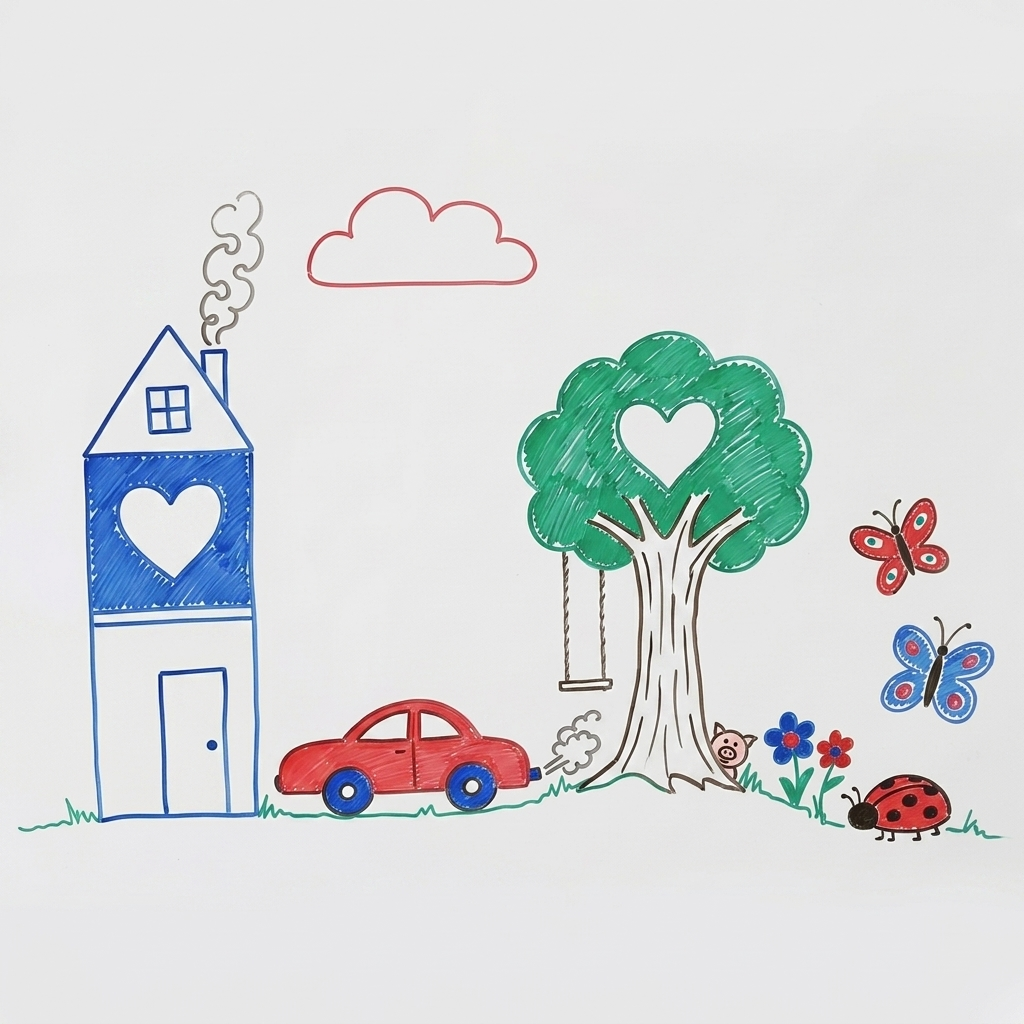
\includegraphics[width=0.85\linewidth]{vokab_300dpi/whiteboard_sketch.png}
\end{center}

\vspace{1.5cm}
\color{geminiBlue}\hrule height 1.5pt \vspace{0.5em}\color{black}

\section[Grammaire an Ausdréck / Grammaire / Grammar]{Grammaire an Ausdréck \\/ Grammaire et Expressions \\/ Grammar and Expressions}

\subsection*{1. Lokal Prepositiounen mat dem Dativ (Prepositions of Place with Dative)}

Am Lëtzebuergeschen verlaangen d'Prepositiounen vum Ort (place) den \textbf{Dativ} fir eng Positioun (Stellung ouni Bewegung) ze beschreiwen. Hei sinn déi wichtegst Prepositiounen mat hiren Dativ-Formen: \\
\textit{En luxembourgeois, les prépositions de lieu exigent le datif pour décrire une position (état sans mouvement). Voici les prépositions les plus importantes avec leurs formes au datif : / In Luxembourgish, prepositions of place govern the dative case to describe a position (state without movement). Here are the most important prepositions with their dative forms:}

\begin{itemize}
    \item \textbf{lénks vum / riets vum} (à gauche de / à droite de - to the left of / to the right of): \\
    \textit{Français : La préposition \textbf{vun} se contracte avec l'article au datif : / English: The preposition \textbf{vun} contracts with the article in the dative case:}
    \begin{itemize}
        \item \textit{vun dem} (masc./neut.) $\rightarrow$ \textbf{vum} (e.g., \textit{lénks vum Bam}, \textit{riets vum Haus})
        \item \textit{vun der} (fem.) $\rightarrow$ \textbf{vun der} (e.g., \textit{riets vun der Dier})
    \end{itemize}
    
    \item \textbf{an der Mëtt} (au milieu - in the middle): \\
    \textit{Français : Le mot \textbf{Mëtt} est féminin. Au datif, l'article devient \textbf{der} : / English: The word \textbf{Mëtt} is feminine. In the dative case, the article becomes \textbf{der}:}
    \begin{itemize}
        \item \textit{an der Mëtt vum Bild} (au milieu de l'image / in the middle of the picture).
    \end{itemize}
    
    \item \textbf{virun / hannert} (devant / derrière - in front of / behind): \\
    \textit{Français : \textbf{virun} s'utilise avec le datif. Devant un consonne, il se contracte souvent en \textbf{virum} : / English: \textbf{virun} governs the dative case. Before a consonant, it often contracts to \textbf{virum}:}
    \begin{itemize}
        \item \textit{virun dem Auto} $\rightarrow$ \textbf{virum Auto} (contracted \textit{virun dem} to \textit{virum} before consonants due to Eifeler Regel).
        \item \textit{hannert dem Haus} (derrière la maison / behind the house).
    \end{itemize}
    
    \item \textbf{niewent / ënner / iwwer} (à côté de / sous / au-dessus de - next to / under / above): \\
    \textit{Français : Ces prépositions régissent également le datif. Pour \textbf{ënner} et \textbf{iwwer}, il existe des variantes régionales se terminant par un "t" : \textbf{ënnert} et \textbf{iwwert} : / English: These prepositions also govern the dative case. For \textbf{ënner} and \textbf{iwwer}, there are regional variants ending with a "t": \textbf{ënnert} and \textbf{iwwert}:}
    \begin{itemize}
        \item \textbf{niewent} (also: \textbf{niewen}, \textbf{nieft}) $\rightarrow$ \textit{niewent dem Bam} (à côté de l'arbre / next to the tree).
        \item \textbf{ënner} (also: \textbf{ënnert}) $\rightarrow$ \textit{ënner dem Bam} / \textit{ënnert dem Bam} (sous l'arbre / under the tree).
        \item \textbf{iwwer} (also: \textbf{iwwert}) $\rightarrow$ \textit{iwwer dem Bam} / \textit{iwwert dem Bam} (au-dessus de l'arbre / above the tree).
    \end{itemize}
    
    \item \textbf{tëschent / zwëschent} (entre - between): \\
    \textit{Français : Les deux formes sont utilisées, mais \textbf{tëschent} et \textbf{tëscht} sont les plus courantes : / English: Both forms are used, but \textbf{tëschent} and \textbf{tëscht} are the most common:}
    \begin{itemize}
        \item \textbf{tëschent} (also: \textbf{tëscht}, \textbf{tëschen}) $\rightarrow$ \textit{tëschent dem Haus an dem Bam} (entre la maison et l'arbre / between the house and the tree).
    \end{itemize}
\end{itemize}

\subsection*{2. Zesummeklappung vu Prepositiounen mat dem Artikel / Contraction des prépositions avec l'article / Contraction of Prepositions with the Article}

Wann d'Prepositioun op e Konsonant stéisst, gëtt de finalen `-n` heiansdo geläscht oder d'Wuert gëtt mat dem Artikel zesummegeluecht: \\
\textit{Lorsqu'une préposition précède une consonne, le "-n" final est parfois élidé ou le mot est contracté avec l'article : / When a preposition precedes a consonant, the final "-n" is sometimes dropped or the word contracts with the article:}
\begin{itemize}
    \item \textbf{vun dem} $\rightarrow$ \textbf{vum} (ëmmer zesummegeluecht: \textit{vum Bam}, \textit{vum Haus}).
    \item \textbf{virun dem} $\rightarrow$ \textbf{virum} (contracted before a consonant, keeping the `-n` before a vowel or `n, d, t, z, h` if split, e.g., \textit{virun dem Auto} vs \textit{virum Bam}).
    \item \textbf{an dem} $\rightarrow$ \textbf{am} (e.g., \textit{am Bam}, \textit{am Haus}).
\end{itemize}

\subsection*{3. De Witz vum "Dag" géint den "Daach"}

Am Lëtzebuergeschen ginn d'Wierder \textbf{Dag} (journée / day) an \textbf{Daach} (toit / roof) an der alldeeglecher Aussprooch identesch ausgeschwat (béid enden mat engem mëllen Frikativ \texttt{[da:x]}). Dëst féiert dacks zu engem klassesche Wuertspill fir Leit déi d'Sprooch léieren: \\
\textit{En luxembourgeois, les mots \textbf{Dag} (journée) et \textbf{Daach} (toit) sont prononcés de manière identique dans la langue parlée quotidienne (se terminant tous deux par la fricative douce \texttt{[da:x]}). Cela conduit souvent à un jeu de mots classique pour les apprenants : / In Luxembourgish, the words \textbf{Dag} (day) and \textbf{Daach} (roof) are pronounced identically in daily spoken language (both ending with the soft fricative \texttt{[da:x]}). This often leads to a classic pun for learners:}

\begin{center}
    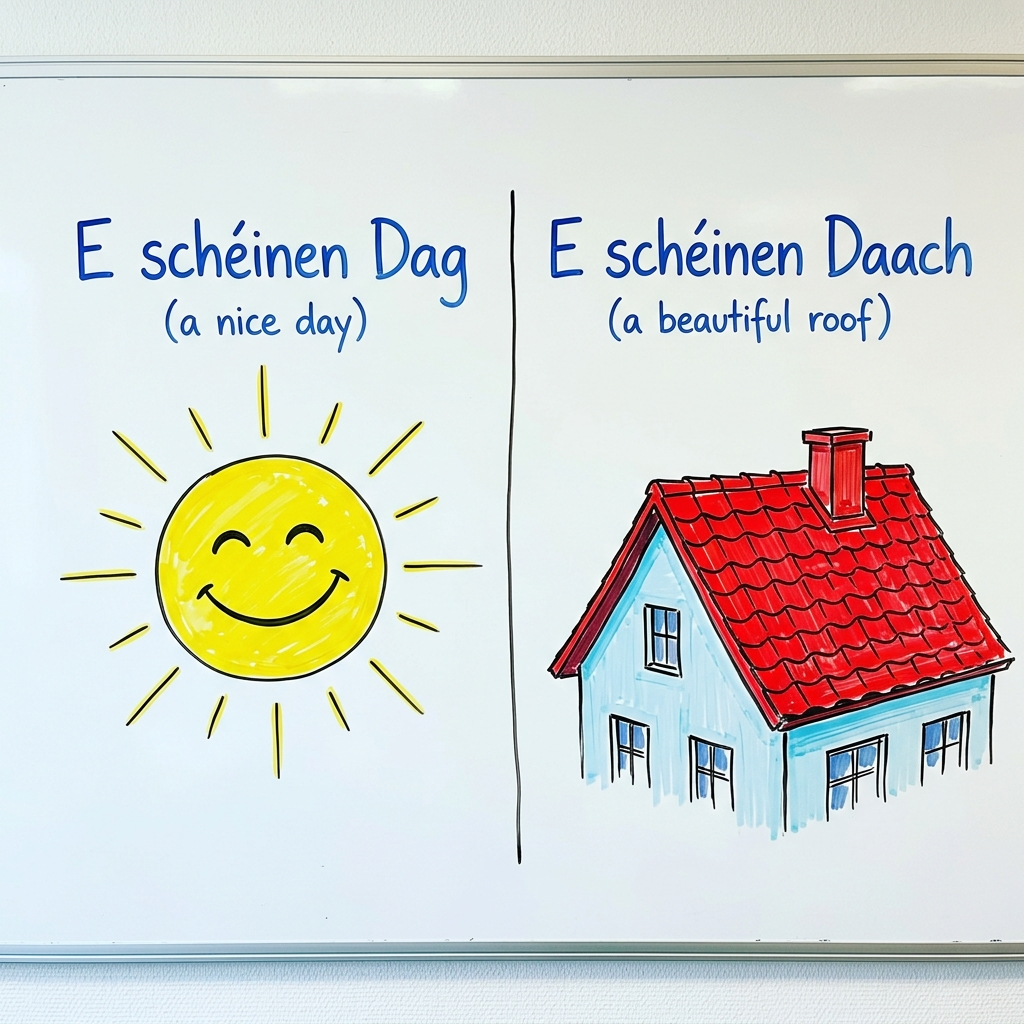
\includegraphics[width=0.7\linewidth]{vokab_300dpi/dag_vs_daach_joke.png}
\end{center}

\begin{itemize}
    \item \textbf{e schéinen Dag} (Pl.: d'Deeg) $\rightarrow$ have a nice day / bonne journée.
    \item \textbf{e schéinen Daach} (Pl.: d'Diech) $\rightarrow$ a beautiful roof / un beau toit.
\end{itemize}
Wann een Iech wënscht: \textit{"E schéinen Daach!"}, wëll hien Iech kee schéinen Daach op Äert Haus wënschen, mee hie wënscht Iech einfach e \textbf{schéinen Dag}!

\vspace{1.5cm}
\color{geminiBlue}\hrule height 1.5pt \vspace{0.5em}\color{black}

\section[Vokabulär: Neit Wierderbuch]{Vokabulär: Neit Wierderbuch \\/ Nouveau Vocabulaire Illustré \\/ New Illustrated Vocabulary}

\begin{itemize}
    \item \textbf{de Bam} (Pl.: de Beem) $\rightarrow$ l'arbre (the tree)
    \item \textbf{d'Haus} (Pl.: d'Haiser) $\rightarrow$ la maison (the house)
    \item \textbf{den Auto} (Pl.: d'Autoen) $\rightarrow$ la voiture (the car)
    \item \textbf{d'Dier} (Pl.: d'Dieren) $\rightarrow$ la porte (the door)
    \item \textbf{d'Wollek} (Pl.: d'Wolleken) $\rightarrow$ le nuage (the cloud)
    \item \textbf{de Päiperlek} (Pl.: de Päiperleken) $\rightarrow$ le papillon (the butterfly)
    \item \textbf{d'Blumm} (Pl.: d'Blummen) $\rightarrow$ la fleur (the flower)
    \item \textbf{d'Himmelsdéierchen} (Pl.: d'Himmelsdéiercher) $\rightarrow$ la coccinelle (the ladybug)
    \item \textbf{d'Schaukel} (Pl.: d'Schaukelen) $\rightarrow$ la balançoire (the swing)
    \item \textbf{d'Klunsch} (Pl.: d'Klunschen) $\rightarrow$ la balançoire (the swing)
    \item \textbf{d'Häerz} (Pl.: d'Häerzer) $\rightarrow$ le cœur (the heart)
    \item \textbf{den Daach} (Pl.: d'Diech) $\rightarrow$ le toit (the roof)
    \item \textbf{de Capybara} (Pl.: de Capybaraen) $\rightarrow$ le capybara (the capybara)
    \item \textbf{d'Schwäin} (Pl.: d'Schwäin) $\rightarrow$ le cochon (the pig)
    \item \textbf{de Buschauffer} (Pl.: de Buschaufferen) $\rightarrow$ le chauffeur de bus (the bus driver)
    \item \textbf{d'Botzfra} (Pl.: d'Botzfraen) $\rightarrow$ la femme de ménage (the cleaning lady)
    \item \textbf{niewent} (also: \textbf{niewen}, \textbf{nieft}) (prep.) $\rightarrow$ à côté de (next to)
    \item \textbf{ënner} (also: \textbf{ënnert}) (prep.) $\rightarrow$ sous (under)
    \item \textbf{iwwer} (also: \textbf{iwwert}) (prep.) $\rightarrow$ sur, au-dessus de (over, above)
    \item \textbf{tëschent} (also: \textbf{tëscht}, \textbf{tëschen}) (prep.) $\rightarrow$ entre (between)
    \item \textbf{pensionéiert} (adj.) $\rightarrow$ retraité, en pension (retired)
    \item \textbf{e schéinen Dag} (Pl.: d'Deeg) $\rightarrow$ une belle journée (a nice day)
\end{itemize}

\vspace{1.5em}

\begin{center}
    \begin{minipage}[t]{0.48\textwidth}
        \centering
        \textbf{E Haus}
        \vspace{0.5em}
        \framebox{\parbox{0.9\linewidth}{\centering
            \vspace{0.5cm}
            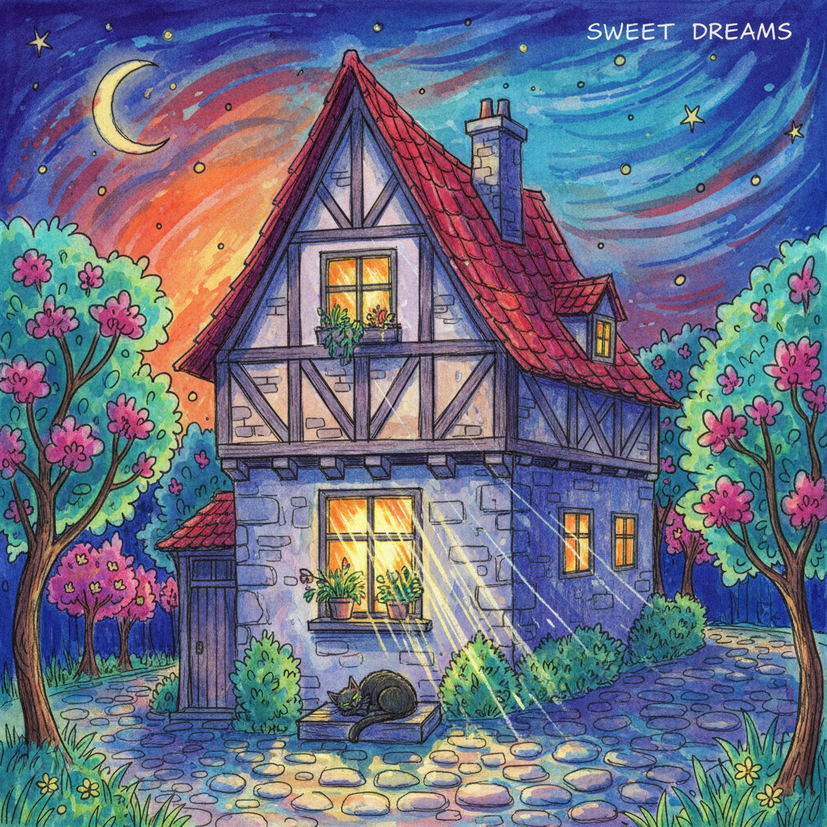
\includegraphics[width=0.9\linewidth]{vokab_300dpi/haus.png} \\
            \small\textit{D'Haus (La maison / The house)}
            \vspace{0.5cm}
        }}
    \end{minipage}
    \hfill
    \begin{minipage}[t]{0.48\textwidth}
        \centering
        \textbf{En Auto}
        \vspace{0.5em}
        \framebox{\parbox{0.9\linewidth}{\centering
            \vspace{0.5cm}
            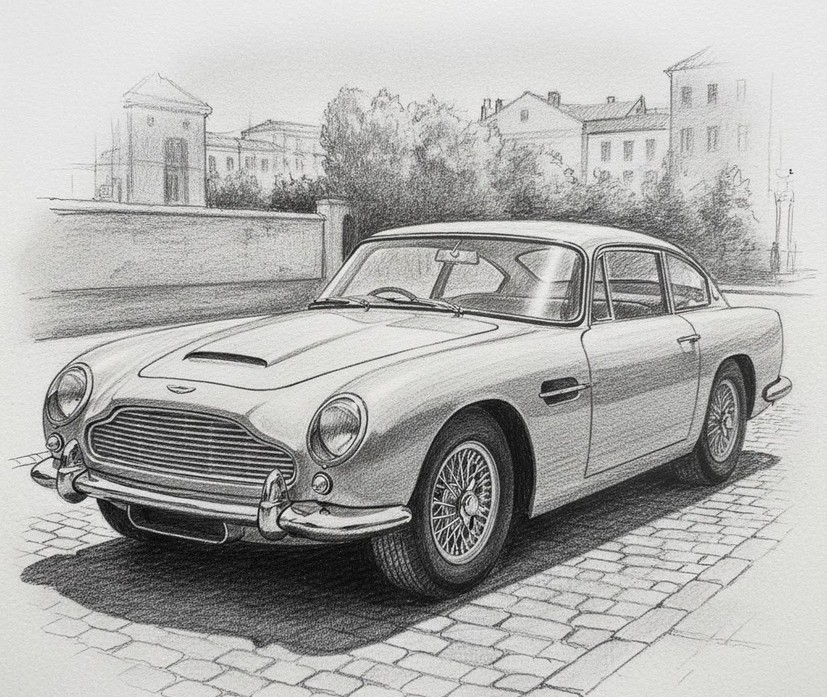
\includegraphics[width=0.9\linewidth]{vokab_300dpi/auto.jpg} \\
            \small\textit{Den Auto (La voiture / The car)}
            \vspace{0.5cm}
        }}
    \end{minipage}
    
    \vspace{1.5em}
    
    \begin{minipage}[t]{0.48\textwidth}
        \centering
        \textbf{Eng Dier}
        \vspace{0.5em}
        \framebox{\parbox{0.9\linewidth}{\centering
            \vspace{0.5cm}
            
\includegraphics[width=0.9\linewidth]{vokab_300dpi/dier.png} \\
            \small\textit{D'Dier (La porte / The door)}
            \vspace{0.5cm}
        }}
    \end{minipage}
    \hfill
    \begin{minipage}[t]{0.48\textwidth}
        \centering
        \textbf{E Schwäin}
        \vspace{0.5em}
        \framebox{\parbox{0.9\linewidth}{\centering
            \vspace{0.5cm}
            
\includegraphics[width=0.9\linewidth]{vokab_300dpi/schwaein.png} \\
            \small\textit{D'Schwäin (Le cochon / The pig)}
            \vspace{0.5cm}
        }}
    \end{minipage}

    \vspace{1.5em}
    
    \begin{minipage}[t]{0.48\textwidth}
        \centering
        \textbf{Eng Wollek}
        \vspace{0.5em}
        \framebox{\parbox{0.9\linewidth}{\centering
            \vspace{0.5cm}
            
\includegraphics[width=0.9\linewidth]{vokab_300dpi/wollek.png} \\
            \small\textit{d'Wollek (Le nuage / The cloud)}
            \vspace{0.5cm}
        }}
    \end{minipage}
    \hfill
    \begin{minipage}[t]{0.48\textwidth}
        \centering
        \textbf{En Himmelsdéierchen}
        \vspace{0.5em}
        \framebox{\parbox{0.9\linewidth}{\centering
            \vspace{0.5cm}
            
\includegraphics[width=0.9\linewidth]{vokab_300dpi/himmelsdeierchen.png} \\
            \small\textit{d'Himmelsdéierchen (La coccinelle / The ladybug)}
            \vspace{0.5cm}
        }}
    \end{minipage}

    \vspace{1.5em}
    
    \begin{minipage}[t]{0.48\textwidth}
        \centering
        \textbf{Eng Schaukel / Eng Klunsch}
        \vspace{0.5em}
        \framebox{\parbox{0.9\linewidth}{\centering
            \vspace{0.5cm}
            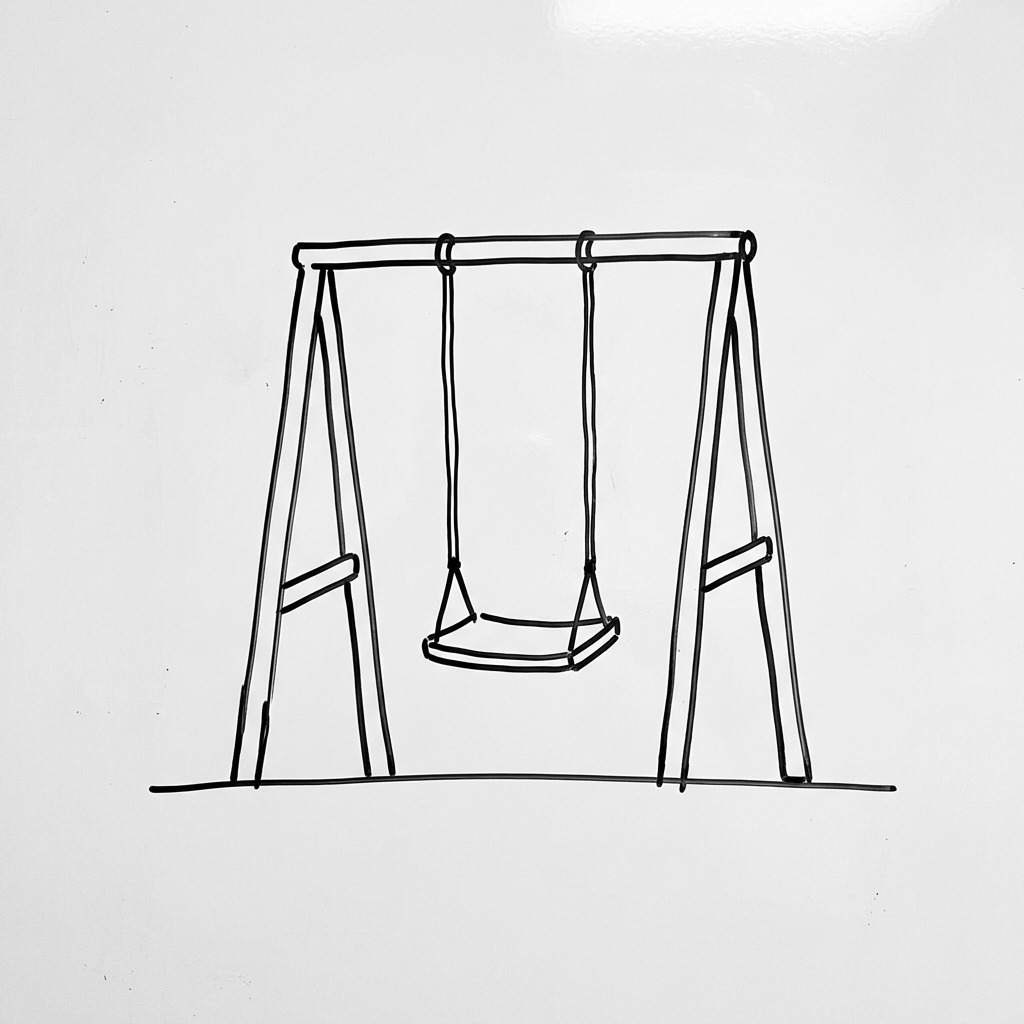
\includegraphics[width=0.9\linewidth]{vokab_300dpi/schaukel.png} \\
            \small\textit{d'Schaukel / d'Klunsch (La balançoire / The swing)}
            \vspace{0.5cm}
        }}
    \end{minipage}
    \hfill
    \begin{minipage}[t]{0.48\textwidth}
        \centering
        \textbf{E Päiperlek}
        \vspace{0.5em}
        \framebox{\parbox{0.9\linewidth}{\centering
            \vspace{0.5cm}
            
\includegraphics[width=0.9\linewidth]{vokab_300dpi/paiperlek.png} \\
            \small\textit{de Päiperlek (Le papillon / The butterfly)}
            \vspace{0.5cm}
        }}
    \end{minipage}

    \vspace{1.5em}
    
    \begin{minipage}[t]{0.48\textwidth}
        \centering
        \textbf{En Häerz}
        \vspace{0.5em}
        \framebox{\parbox{0.9\linewidth}{\centering
            \vspace{0.5cm}
            
\includegraphics[width=0.9\linewidth]{vokab_300dpi/haerz.png} \\
            \small\textit{d'Häerz (Le cœur / The heart)}
            \vspace{0.5cm}
        }}
    \end{minipage}
\end{center}
